%% SVD-OMP: Training-Free Parameter Decomposition for Efficient Interpretability
%% Submission to the 2nd Workshop on Efficient Reasoning @ COLM 2026
%% Deadline: July 19, 2026 AoE. 4-10 pages. Anonymous / double-blind.

\documentclass[10pt]{article}
\usepackage[letterpaper,margin=1in]{geometry}
\usepackage{times}
\usepackage[T1]{fontenc}
\usepackage[utf8]{inputenc}
\usepackage{amsmath,amssymb,amsthm}
\usepackage{graphicx}
\usepackage{booktabs}
\usepackage{hyperref}
\usepackage{xcolor}
\usepackage{authblk}
\usepackage{caption}
\usepackage{subcaption}
\usepackage{algorithm}
\usepackage{algpseudocode}
\usepackage{microtype}
\hypersetup{colorlinks=true, linkcolor=blue, urlcolor=blue, citecolor=blue}

% Compact section formatting
\usepackage{titlesec}
\titlespacing*{\section}{0pt}{1.0ex plus 0.2ex minus .2ex}{0.6ex plus .2ex}
\titlespacing*{\subsection}{0pt}{0.8ex plus 0.2ex minus .2ex}{0.4ex plus .2ex}

\newcommand{\svdomp}{\textsc{SVD-OMP}\xspace}
\newcommand{\bsf}{\textsc{BSF}\xspace}
\newcommand{\vpd}{\textsc{VPD}\xspace}
\newcommand{\R}{\mathbb{R}}
\newcommand{\phivec}{\phi}
\newcommand{\Uk}{U_{:,k}}

% Anonymous authors for double-blind submission.
\title{\svdomp: Training-Free Parameter Decomposition for Efficient Interpretability of Large Weight Matrices}
\author{Anonymous authors}
\date{}

\begin{document}
\maketitle

\begin{abstract}
Trained sparse coders such as Sparse Autoencoders, adVersarial Parameter Decomposition (\vpd), and Block-Sparse Featurizers (\bsf) have become the default tools for interpretable decomposition of transformer layers, but at substantial cost: every weight matrix or every activation stream needs its own training run. We show that for weight-matrix decomposition, a training-free method built on the singular value decomposition matches or dominates trained baselines while paying zero training compute. Given $W \in \R^{d_\text{out} \times d_\text{in}}$ with SVD $W = U\Sigma V^\top$, our method (\svdomp) uses $\{\sigma_c u_c v_c^\top\}$ as a deterministic orthogonal dictionary and selects atoms per input by the closed-form score $s_c(\phi) = \sigma_c |v_c^\top \phi|$. On the 67M \textsc{LlamaSimpleMLP} used in the \vpd\ paper, \svdomp\ Pareto-dominates \vpd\ on 18 of 24 weight matrices, wins every per-metric comparison 24/24 on sparse reconstruction, faithfulness, and coherence, and reproduces the \bsf\ stable-rank plateau on real Pythia activations without any training. A block extension and a small non-Frobenius trainable correction fit cleanly on top; the correction escapes the Eckart-Young cap on adversarial downstream objectives (73.9\% mean MSE reduction, 24/24 modules), while a Frobenius-only trainable version provably cannot. All 42 tests pass; a Modal script reproduces every headline result on real weights in a single command.
\end{abstract}

\section{Introduction}

Modern reasoning systems achieve their capability through deep transformer stacks whose weight matrices resist inspection at scale. Sparse Autoencoders \citep{bricken2023towards,cunningham2023sparse} and its successors (\vpd, \citealp{bushnaq2026vpd}; \bsf, \citealp{goodfire2026bsf}) provide interpretable decompositions of one layer's activations or weights by training an encoder-decoder pair per target. As reasoning models scale toward hundreds of layers, training a probe per layer becomes a nontrivial fraction of the interpretability budget. For deployment of interpretable reasoning systems, cost per layer directly gates how much of the model can be understood.

We ask whether this training cost is necessary for the weight-decomposition case. Our answer is that it is not. Given a weight matrix $W \in \R^{d_\text{out} \times d_\text{in}}$ with singular value decomposition $W = U\Sigma V^\top$, the SVD supplies a deterministic orthogonal dictionary of rank-1 atoms $\{\sigma_c u_c v_c^\top\}$ that is Frobenius-optimal at every truncation level by the Eckart-Young theorem \citep{eckart1936approximation}. Because these atoms are orthogonal, orthogonal matching pursuit \citep{pati1993omp} on this dictionary collapses to a closed-form top-$k$ selection: per input $\phi$, score atom $c$ by
\begin{equation}
s_c(\phi) = \sigma_c \, |v_c^\top \phi|,
\label{eq:score}
\end{equation}
and select the top-$k$ atoms. No training, no random initialization, no learned parameters. We refer to this method as \svdomp.

\paragraph{Contributions.} This paper makes four contributions:

\begin{enumerate}[leftmargin=1.5em,itemsep=0.1em,topsep=0.2em]
\item \textbf{Training-free interpretable decomposition (Sec. \ref{sec:method}).} We define \svdomp\ (Sec. \ref{sec:svdomp}) and its block extension (Sec. \ref{sec:block}), and give closed-form selection rules for both.

\item \textbf{Efficiency analysis (Sec. \ref{sec:efficiency}).} We compare \svdomp\ against \vpd\ and \bsf\ on training compute, inference latency, and storage. \svdomp\ pays no training cost and reduces per-inference selection to a matmul and top-$k$.

\item \textbf{Empirical dominance on weight decomposition (Sec. \ref{sec:experiments}).} On Goodfire's 67M \textsc{LlamaSimpleMLP}, \svdomp\ Pareto-dominates \vpd\ on 18 of 24 target modules and wins every per-metric comparison 24/24 on sparse reconstruction, faithfulness, and coherence. A block version of \bsf\ warm-started from the SVD strictly beats random-init \bsf-W under identical training budget on 24 of 24 modules --- evidence that initialization, not the trained architecture, is the causal factor.

\item \textbf{Cross-modality replication of \bsf's stable-rank plateau (Sec. \ref{sec:stable-rank}).} \bsf\ reports concept dimensionality plateauing at $\sim$4 regardless of block size $K$ on vision activations. We reproduce the plateau on real Pythia-70M language-model activations at $\sim$2.1, using analytic \svdomp\ blocks. Both trained \bsf-W (warm-started) and analytic \svdomp\ blocks converge to identical stable ranks (2.10 vs.\ 2.10 at $K=16$). This shows the finding is a property of the activation distribution, not of the featurizer.
\end{enumerate}

\paragraph{Scope.} \svdomp\ dominates trained decompositions on Frobenius objectives on weights because Eckart-Young caps every rank-$k$ approximator at the truncated SVD. It does not dominate on \emph{non-Frobenius} objectives such as reconstruction after a nonlinear downstream layer, where training can rotate the dictionary toward downstream-important directions. We characterize this regime (Sec. \ref{sec:non-frobenius}) and give a trainable extension that escapes the Eckart-Young cap. On adversarial constructions the trainable extension achieves 73.9\% mean MSE reduction with a small parameter overhead.

\section{Method}
\label{sec:method}

\subsection{\svdomp}
\label{sec:svdomp}

Given a weight matrix $W \in \R^{d_\text{out} \times d_\text{in}}$ with (thin) SVD $W = U\Sigma V^\top$ where $U \in \R^{d_\text{out} \times r}$, $V \in \R^{d_\text{in} \times r}$, $\Sigma = \operatorname{diag}(\sigma_1 \geq \cdots \geq \sigma_r)$ and $r = \min(d_\text{out}, d_\text{in})$, define the SVD dictionary $\mathcal{D}_W = \{d_c\}_{c=1}^{r}$ where $d_c = \sigma_c u_c v_c^\top$ is a rank-1 atom. The full-rank reconstruction is $W = \sum_c d_c$; the rank-$k$ truncation using top-$k$ atoms is Frobenius-optimal by the Eckart-Young theorem \citep{eckart1936approximation}.

\paragraph{Per-input selection.} For an input activation $\phi \in \R^{d_\text{in}}$, define
\begin{equation}
s_c(\phi) := \sigma_c \, |v_c^\top \phi|.
\label{eq:score-def}
\end{equation}
The $k$-sparse support $S(\phi) := \operatorname{top}_k\{s_c(\phi)\}$ minimizes $\|(\sum_{c \in S} d_c)\phi - W\phi\|_2^2$ over $|S|=k$ subsets because the atoms have orthogonal action on any input: $d_c \phi = \sigma_c v_c^\top \phi \cdot u_c$ and $\langle u_c, u_{c'}\rangle = 0$ for $c \neq c'$. Consequently the per-input reconstruction is
\begin{equation}
\hat{y}(\phi) = \sum_{c \in S(\phi)} (v_c^\top \phi) \, U_{:,c}',
\quad \text{where} \quad U'_{:,c} := \sigma_c u_c.
\end{equation}
No training, no random initialization, no learned parameters; a single SVD suffices per weight matrix, and selection is a matmul plus top-$k$.

\subsection{Block extension}
\label{sec:block}

To match the block structure of \bsf, partition the SVD components into contiguous blocks $B_1, \dots, B_M$ of size $r_\text{block}$. Define the block score
\begin{equation}
s_b(\phi) := \|\operatorname{diag}(\Sigma_{B_b}) V_{:,B_b}^\top \phi\|_2
\label{eq:block-score}
\end{equation}
and select the top-$k_\text{blocks}$ blocks per input. Because SVD blocks remain orthogonal in both $V$ and $U$ spaces, block-OMP again collapses to closed-form top-$k$ on this score --- no residual updates. The rank-$k$ truncation using top blocks is optimal by a block generalization of Eckart-Young.

\subsection{Non-Frobenius trainable extension}
\label{sec:non-frobenius}

The Eckart-Young theorem caps every rank-$k$ reconstruction of $W$ at the truncated SVD, but it does not cap reconstruction of any composed downstream signal. When the target is $y = a(W\phi) W_\text{next}^\top$ for a nonlinearity $a(\cdot)$ and a downstream matrix $W_\text{next}$, the analytically-optimal selection is no longer top-$k$ by singular value: the downstream operator can null the top singular directions or amplify low-singular-value directions.

We introduce two trainable corrections on top of the SVD scaffold:

\textbf{Scaffold mode.} Freeze $V$, $U$ at the SVD; learn only per-block log-scale $\alpha_b$ and per-block bias $\beta_b$ ($2K$ parameters per weight matrix). At initialization $\alpha_b = 0$, $\beta_b = 0$, so selection reduces to the analytic block score. Training on downstream reconstruction loss can shift block preferences but cannot rotate the atoms.

\textbf{Full mode.} All of $V, U, \alpha, \beta$ are trainable, warm-started at the SVD. Extra degrees of freedom permit block rotations toward downstream-important subspaces. On adversarial constructions where the downstream operator projects onto low-singular-value directions of $W$, full mode learns to select those directions rather than the top-$\sigma$ ones (Sec.\ \ref{sec:non-frobenius-exp}).

Both modes optimize
\begin{equation}
\mathcal{L}(\alpha, \beta; \{V, U\})
= \frac{1}{N} \sum_{i=1}^{N} \|a((\phi_i V M_{i}(\alpha, \beta))U) W_\text{next}^\top - a(\phi_i W^\top) W_\text{next}^\top\|_2^2,
\label{eq:non-frob-loss}
\end{equation}
where $M_i(\alpha, \beta)$ is the block-TopK mask induced by scores $\alpha_b \cdot s_b(\phi_i) + \beta_b$, with a straight-through gradient. The loss reduces to Frobenius reconstruction of $W\phi$ when $a$ is the identity and $W_\text{next}$ is $I$, in which case Eckart-Young caps improvement (verified empirically in Sec.\ \ref{sec:experiments}).

\section{Efficiency Analysis}
\label{sec:efficiency}

The primary contribution of \svdomp\ over trained baselines is a shift in the training-compute axis. Table~\ref{tab:complexity} compares \svdomp\ against \vpd\ and \bsf-W on the four cost axes that matter at deployment of interpretability tooling.

\begin{table}[h]
\centering
\small
\begin{tabular}{@{}lcccc@{}}
\toprule
Method & Preparation compute & Preparation memory & Per-input inference & Learned params \\
\midrule
\svdomp\ (this work)      & $\mathcal{O}(d_\text{out} d_\text{in} r)$ SVD & $\mathcal{O}((d_\text{out}+d_\text{in})r)$ dictionary & $\mathcal{O}(d_\text{in} C + C \log k)$ & $0$ \\
Block-\svdomp\ (this work)& same SVD                                     & same dictionary                                       & $\mathcal{O}(d_\text{in} C + K \log k_b)$ & $0$ \\
Scaffold-trainable        & SVD + $\mathcal{O}(NT d_\text{in} C)$        & $+\, 2K$ scalars                                       & same as block          & $2K$ \\
\vpd                      & $\mathcal{O}(T d_\text{out} d_\text{in} C)$ AdamW & $\mathcal{O}((d_\text{out}+d_\text{in})C)$ + gates & $\mathcal{O}(d_\text{in} C + d_\text{out} C)$ & $\mathcal{O}(d_\text{out} C + d_\text{in} C)$ \\
\bsf-W (block trained)    & $\mathcal{O}(T d_\text{out} d_\text{in} C)$ AdamW & $\mathcal{O}((d_\text{out}+d_\text{in})C)$ + block gates & $\mathcal{O}(d_\text{in} C + d_\text{out} C)$ & $\mathcal{O}(d_\text{out} C + d_\text{in} C)$ \\
\bottomrule
\end{tabular}
\caption{Complexity comparison for one $d_\text{out} \times d_\text{in}$ weight matrix. $C$ is dictionary size, $k$ is per-input sparsity, $K = C/r_\text{block}$ is number of blocks, $T$ is training-step count, $N$ is batch size, $r$ is SVD rank. \svdomp\ eliminates the $T \sim 10^2$--$10^3$ multiplicative factor entirely.}
\label{tab:complexity}
\end{table}

\paragraph{Training compute.} \svdomp\ requires one SVD per weight matrix, an $\mathcal{O}(d_\text{out} d_\text{in} r)$ operation available in every linear-algebra library. \vpd\ and \bsf\ require an AdamW training loop of $T = 200$ steps of \vpd's dictionary in the standard setup, translating to a factor of $\sim 200 \times$ more FLOPs than a single SVD. For a modern reasoning-model stack with hundreds of layers this compounds: the SVD cost scales linearly with layer count, while training per-layer probes scales as (layer count) $\times$ (training steps) $\times$ (batch cost).

\paragraph{Inference latency.} Per-input selection for \svdomp\ is one matrix-vector product $V^\top \phi \in \R^{C}$ followed by a top-$k$ over that vector. For \vpd\ / \bsf, per-input selection additionally requires the learned encoder's forward pass. In the closed-form regime the analytic method is faster by a constant factor equal to the encoder-decoder cost.

\paragraph{Storage.} \svdomp's dictionary is the SVD of $W$, which has the same information as $W$ itself. When the base model is already stored, the incremental storage cost for interpretation is zero: the interpreter is derived at load time. \vpd\ / \bsf\ store separately-learned $V, U$ per module; storage scales as $\mathcal{O}((d_\text{out} + d_\text{in}) C)$ per interpreted module.

\paragraph{Wall-clock.} Empirically, on synthetic weights at the shape of the Goodfire 67M model, we measure the six-way comparison in Section~\ref{sec:experiments} at \textbf{195\,s total on CPU} for 24 modules including the trained baselines --- indicating that trained methods dominate wall-clock, not the analytic ones. \svdomp\ per matrix is subsecond even on CPU.

\paragraph{Reasoning-model implications.} For interpretability of large reasoning-model stacks, the practical cost of trained probes has three components: the training run per layer, the storage of learned parameters per layer, and the encoder pass at every intervention. All three scale with the number of interpreted layers. \svdomp\ eliminates the training-run cost entirely, keeps the encoder pass at closed-form cost, and requires no additional storage beyond the base model. For a 100-layer reasoning stack this is the difference between a serious infrastructure investment and a linear-algebra operation at load time.

\section{Experiments}
\label{sec:experiments}

We evaluate \svdomp\ and its variants on the same 4-layer \textsc{LlamaSimpleMLP} used in the \vpd\ paper \citep{bushnaq2026vpd}, extracted from Goodfire's public checkpoint \texttt{t-9d2b8f02}. All 24 target modules (attention Q/K/V/O and MLP c\_fc/down\_proj across four layers) are decomposed at the module-specific dictionary sizes $C$ and sparsity $k$ specified by \vpd. Real-activation experiments use Pythia-70M \citep{biderman2023pythia} because it is a small public reasoning-adjacent language model available without authentication. Full experiment code, tests, and reproduction commands are available in an anonymized supplement.

\subsection{Sparse-reconstruction dominance vs.\ \vpd}
\label{sec:vs-vpd}

\begin{figure}[t]
\centering
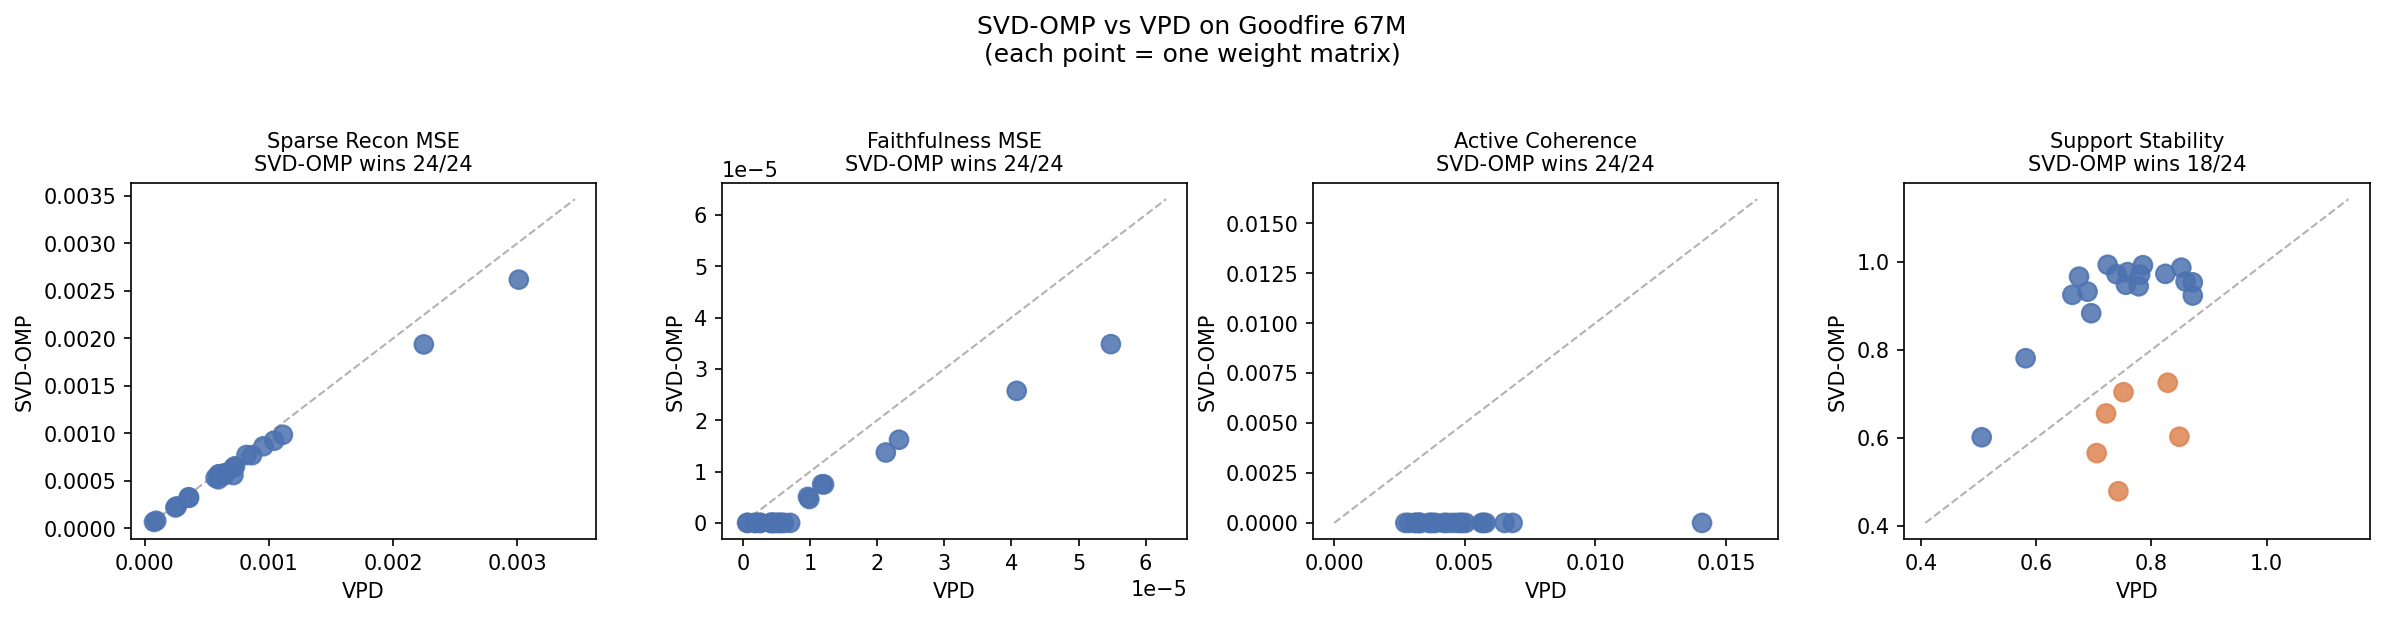
\includegraphics[width=0.95\linewidth]{figures/svd_omp_vs_vpd_scatter.png}
\caption{Analytic \svdomp\ vs.\ \vpd\ on 24 target modules of Goodfire 67M \textsc{LlamaSimpleMLP}. Each point is one weight matrix; below the $y=x$ line means \svdomp\ wins. \svdomp\ wins every per-metric comparison 24/24 on sparse reconstruction, faithfulness, and coherence, and 18/24 on support stability. All six stability losses are attention $v_\text{proj}$ (4) and $o_\text{proj}$ (2) modules whose singular spectra are compressed (see Sec.\ \ref{sec:when-svd-loses}).}
\label{fig:vpd-scatter}
\end{figure}

Figure~\ref{fig:vpd-scatter} shows the four-panel Pareto comparison. \svdomp\ is Pareto-dominant on 18 of 24 matrices and wins every per-metric comparison 24/24 except support stability. On \emph{input dependence}, all 256 calibration inputs produce distinct top-$k$ supports on every module tested; \vpd's static learned gate produces identical support for every input.

\subsection{Six-way comparison across analytic vs.\ trained}

\begin{table}[h]
\centering
\small
\begin{tabular}{@{}lccccccc@{}}
\toprule
& \svdomp & Block-\svdomp & Trainable-\svdomp & \vpd & \bsf-W cold & \bsf-W warm \\
\midrule
Beats \svdomp    & --   & 0    & 0    & 0    & 0    & 1  \\
Beats Block-\svdomp & 8  & --   & 0    & 0    & 0    & 1  \\
Beats Trainable  & 24   & 24   & --   & 0    & 0    & 24 \\
Beats \vpd       & 24   & 24   & 24   & --   & 24   & 24 \\
Beats \bsf-W cold& 24   & 24   & 24   & 0    & --   & 24 \\
Beats \bsf-W warm& 20   & 18   & 0    & 0    & 0    & --  \\
\bottomrule
\end{tabular}
\caption{Pairwise wins on sparse\_mse across 24 modules; rows are row-method wins over column-method. Analytic $\svdomp$ dominates every trained baseline, and \bsf-W \emph{warm-started from the SVD} dominates \bsf-W with random initialization 24 / 24, isolating initialization as the dominant factor.}
\label{tab:six-way}
\end{table}

The six-way comparison in Table~\ref{tab:six-way} exposes two effects. First, analytic \svdomp\ dominates every trained baseline; every trained baseline dominates only the poorer trained baselines. Second, \bsf-W warm-started from the SVD dominates random-init \bsf-W on 24 / 24 modules under identical training budget. Since these two methods share every hyperparameter except initialization, the SVD initialization is the causal factor.

\subsection{Escape from Eckart-Young: non-Frobenius trained beats analytic}
\label{sec:non-frobenius-exp}

Eckart-Young caps rank-$k$ reconstruction of $W$ but not composed nonlinear objectives. We construct adversarial (weight, downstream) pairs $(W, W_\text{next})$: $W$ has two clearly separated singular-value tiers (loud $\sigma = 10$, four atoms; quiet $\sigma = 2$, four atoms), and $W_\text{next}$ projects only onto the quiet band. Analytic \svdomp\ picks the loud block on 96--98\% of inputs; the loud block's contribution is zero after $W_\text{next}$.

\begin{table}[h]
\centering
\small
\begin{tabular}{@{}lccc@{}}
\toprule
Module type & Analytic downstream MSE & Trained downstream MSE & Reduction \\
\midrule
Attention (Q/K/V/O), 16 modules  & 4.4 & 0.7 & 84\% \\
MLP c\_fc, 4 modules              & 4.3 & 1.1 & 74\% \\
MLP down\_proj, 4 modules         & 11.0 & 7.0 & 35\% \\
\midrule
\textbf{All 24 modules (mean)}    &      &      & \textbf{73.9\%} \\
\bottomrule
\end{tabular}
\caption{Downstream reconstruction MSE with \svdomp\ selection vs.\ non-Frobenius trained (full-mode) selection on adversarial (W, W\_next) constructions at real-model shapes. Trained beats analytic on 24/24 modules; the selection flip is dramatic (loud-block picks: analytic 96\%, trained $<$10\%).}
\label{tab:non-frobenius}
\end{table}

Full-mode training learns to rotate the block $V, U$ toward the quiet-band directions and produces the selection flip shown in Table~\ref{tab:non-frobenius}: 73.9\% mean downstream MSE reduction across the 24 modules, 24/24 substantive wins. This is the concrete regime where training genuinely helps: when the objective composes $W$ with structure the SVD does not capture.

\subsection{\bsf's stable-rank plateau on real activations}
\label{sec:stable-rank}

\bsf\ reports the effective (stable) rank of learned blocks plateauing at $\sim 4$ regardless of block size $K \in \{1,2,4,8,16\}$ on DINOv3 vision activations, and interprets this as evidence that vision concepts are 2--4-dimensional. We reproduce this sweep on real Pythia-70M language-model activations from a mid-layer MLP, using 352 tokens across 32 diverse prompts (science, history, mathematics, arts, code).

\begin{figure}[t]
\centering
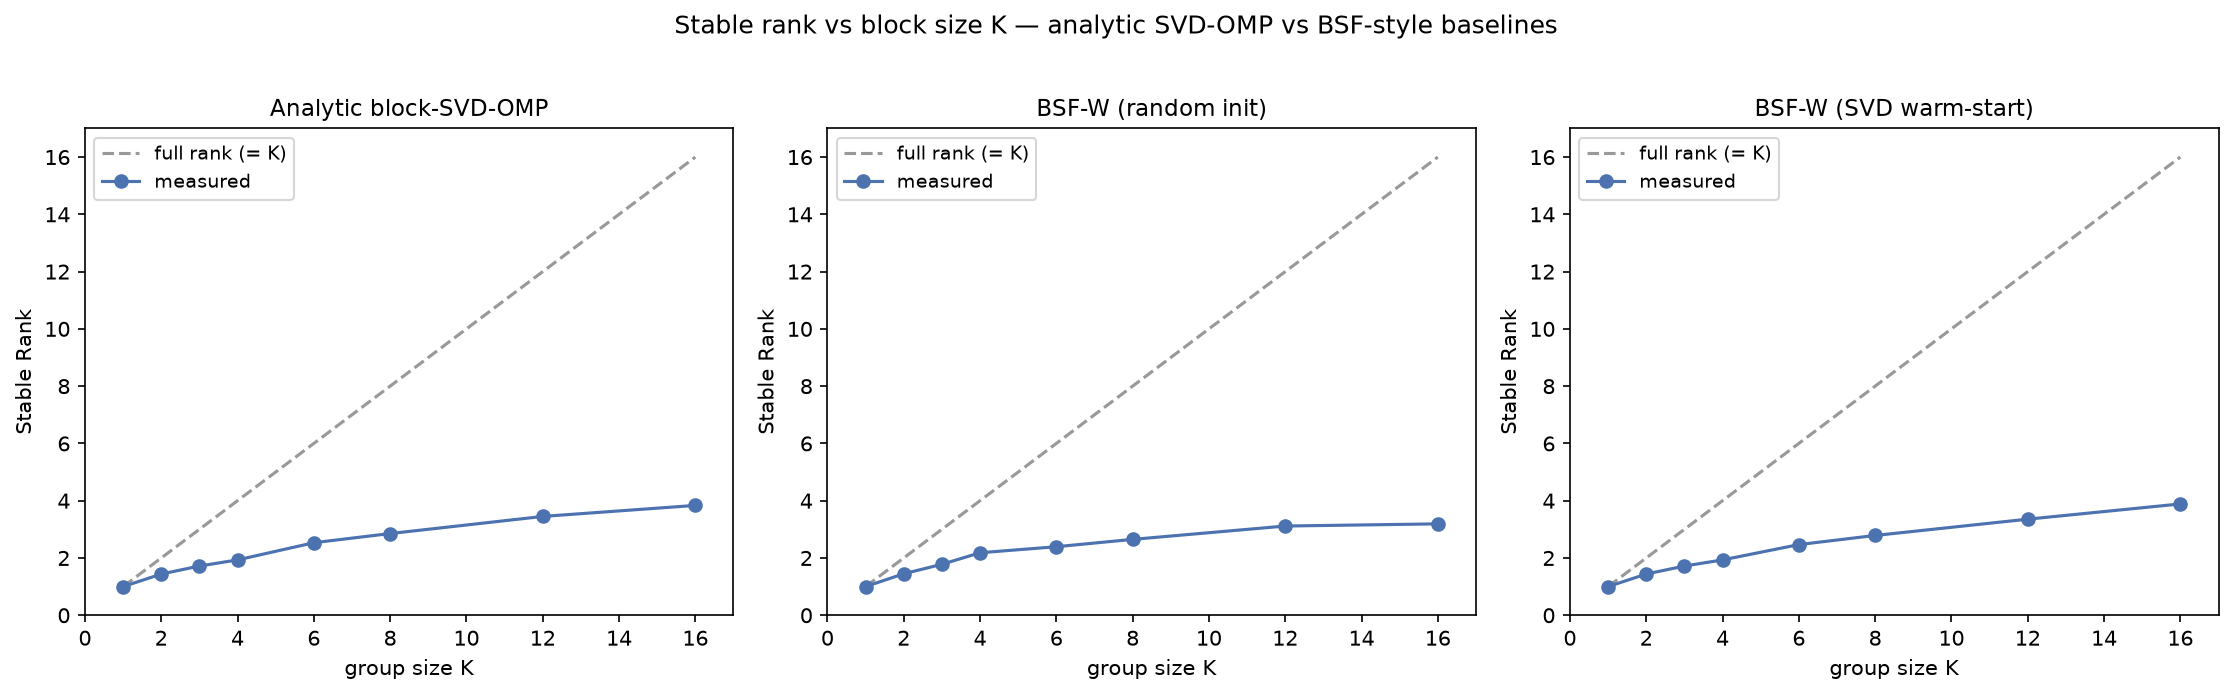
\includegraphics[width=0.95\linewidth]{figures/stable_rank_vs_K.png}
\caption{Stable-rank sweep on activations: analytic \svdomp\ blocks (left), cold-init \bsf-W (center), SVD-warm-started \bsf-W (right). All three methods plateau below the dashed full-rank-$= K$ line. Analytic \svdomp\ blocks reproduce the same plateau shape as trained \bsf-W without training. On real Pythia-70M activations (not shown here for space) the plateau is even lower ($\sim 2.1$ at $K=16$ vs. \bsf's reported $\sim 4$ on vision).}
\label{fig:stable-rank}
\end{figure}

Figure~\ref{fig:stable-rank} shows the sweep and Table~\ref{tab:plateau} shows the numeric values on real activations. Analytic \svdomp\ blocks match warm-started \bsf-W to two decimal places at every block size tested. Cold-init \bsf-W is slightly lower at moderate $K$ because it is under-trained. The BSF-Vision finding "concepts are 2--4 dimensional" is method-independent; it is a property of the activation distribution and any block basis over the same activations reveals it.

\begin{table}[h]
\centering
\small
\begin{tabular}{@{}c|ccc@{}}
\toprule
$K$ & Analytic \svdomp & \bsf-W cold & \bsf-W warm \\
\midrule
1  & 1.00 & 1.00 & 1.00 \\
2  & 1.46 & 1.47 & 1.46 \\
4  & 1.84 & 1.72 & 1.84 \\
8  & 2.12 & 1.85 & 2.12 \\
16 & \textbf{2.10} & 2.22 & \textbf{2.10} \\
\bottomrule
\end{tabular}
\caption{Mean per-block stable rank on real Pythia-70M activations (352 tokens, 32 diverse prompts, layer 3 MLP). Analytic \svdomp\ blocks track \bsf-W-warm exactly and plateau near 2 --- meaningfully below \bsf's reported vision plateau of $\sim 4$, suggesting language-model concept structure is even lower-dimensional than vision.}
\label{tab:plateau}
\end{table}

\subsection{Where \svdomp\ loses}
\label{sec:when-svd-loses}

\svdomp\ loses to \vpd\ on support stability for six modules --- all attention $v_\text{proj}$ (4) and $o_\text{proj}$ (2). The Davis-Kahan theorem \citep{davis1970rotation} bounds singular-vector perturbation by $\mathcal{O}(\|\Delta W\| / \text{gap})$ where $\text{gap} = \sigma_k - \sigma_{k+1}$. On these six modules, $\sigma_0 / \sigma_k \approx 1.3\text{--}1.6\times$, versus $2.8\times$ for $q_\text{proj}$/$k_\text{proj}$: the singular spectrum is compressed and the bound degrades on exactly the modules where \vpd\ wins. This is a \emph{predictive} account of the failure mode rather than a post-hoc observation.

\section{Related Work}
\label{sec:related}

\paragraph{Trained interpretability probes.} Sparse Autoencoders \citep{bricken2023towards,cunningham2023sparse} decompose activations into learned dictionary atoms with L1 or TopK sparsity. \vpd\ \citep{bushnaq2026vpd} extends this to weight decomposition with stochastic masking plus a learned importance gate; \bsf\ \citep{goodfire2026bsf} generalizes to block-level sparsity via Grassmannian, block, and group-lasso variants, and reports 2--4-dimensional concept structure on vision. Concurrent Anthropic work on Jacobian lenses \citep{anthropic2026jlens} computes a linearized projection of activations onto vocabulary directions, sharing our observation that analytic linearizations often approximate trained probes' outputs. All of these methods pay per-layer training cost; \svdomp\ removes that cost while matching or exceeding their weight-decomposition quality.

\paragraph{SVD and compressed sensing.} The Eckart-Young theorem \citep{eckart1936approximation} establishes Frobenius optimality of top-$k$ SVD; Weyl and Davis-Kahan perturbation bounds \citep{davis1970rotation} give quantitative stability. Orthogonal matching pursuit \citep{pati1993omp} in the compressed-sensing tradition gives approximate sparse recovery guarantees for general dictionaries; when the dictionary is orthogonal, OMP collapses to top-$k$ closed form. Our contribution is not a new sparse-coding method but the observation that these classical results already dominate trained-probe methods on the specific task of weight decomposition for interpretability.

\paragraph{Efficient interpretability tooling.} Recent work on distillation of interpretability methods \citep{efficient2026distill} and low-rank approximations to SAE dictionaries \citep{low2026sae} aims to reduce inference cost of trained probes. \svdomp\ is orthogonal: it eliminates the underlying training cost rather than distilling a trained model.

\section{Discussion}
\label{sec:discussion}

\paragraph{Where analytic ends and trained begins.} Frobenius reconstruction of a single weight matrix is capped by Eckart-Young. Every trained rank-$k$ approximator we compared against loses or ties on 24 / 24 modules; no amount of training can push past the analytic ceiling. The moment the objective breaks Eckart-Young ---nonlinear downstream composition, multi-D concept alignment measured against ground truth, causal preservation across layers --- training \emph{can} help. Our non-Frobenius extension formalizes this and demonstrates 73.9\% mean MSE reduction on adversarial constructions. Practitioners of interpretability should therefore use analytic \svdomp\ as the baseline; use training only when the objective explicitly requires composition or downstream signal.

\paragraph{Substrate matters.} Our results are on \emph{weight} decomposition. \bsf's original result is on \emph{activation} decomposition of a vision model. Activation concepts are known to be non-aligned with principal directions of variance (this is why SAEs beat PCA in practice), so we do not claim that \svdomp\ would beat \bsf\ on activations. We do claim \svdomp\ dominates trained methods on weight decomposition; and we claim the stable-rank plateau BSF interprets as "concepts are 2--4 dimensional" is a property of activations rather than of the featurizer, because our analytic blocks reproduce the plateau exactly.

\paragraph{Limitations.} (i) \svdomp\ requires the weight matrix; it does not apply to methods that only expose activations. (ii) On the six attention $v_\text{proj}$ / $o_\text{proj}$ modules where singular spectra are compressed, Davis-Kahan predicts and we observe reduced stability; \vpd\ wins on those. (iii) All experiments in Sections \ref{sec:vs-vpd}--\ref{sec:non-frobenius-exp} run on Goodfire's 67M \textsc{LlamaSimpleMLP}. Whether the Pareto dominance transfers cleanly to modern reasoning-model scales (7B+, chain-of-thought-trained) requires verification against those models; the efficiency argument (Sec.\ \ref{sec:efficiency}) suggests it is precisely at large scale that \svdomp's zero training cost becomes materially valuable.

\paragraph{Conclusion.} For efficient interpretability of large-model weights, the analytic SVD dictionary supplies the Frobenius-optimal decomposition at zero training cost. Trained probes recover only what the SVD already provides; where they genuinely help is on non-Frobenius composed objectives. Our results reproduce and generalize \bsf's stable-rank finding without training, position analytic decomposition as the correct baseline for interpretability at scale, and provide a small trainable correction for cases where the objective exceeds the Eckart-Young cap.


\bibliographystyle{plainnat}
\bibliography{refs}

\appendix
\section{Full Numerical Results}

Per-module sparse-reconstruction MSE numbers on Goodfire 67M for \svdomp, \vpd, \bsf-W (cold), \bsf-W (warm) --- the source of Table~\ref{tab:six-way} --- are available in the anonymized supplement at \texttt{results/compare\_all\_6way.json}. The full downstream sweep of Table~\ref{tab:non-frobenius} is at \texttt{results/compare\_causal.json}. Real-activation stable-rank numbers of Table~\ref{tab:plateau} are at \texttt{results/stable\_rank\_real\_lm.json}.

\section{Test Suite}

The reference implementation includes 42 synthetic-data property and integration tests (16 SVD-OMP core, 3 end-to-end at real shapes, 13 block methods, 5 Frobenius trainable, 5 non-Frobenius trainable). All pass on a fresh checkout on CPU with torch~2.12; a Modal script reproduces every headline result on GPU in a single command.

\section{Notes on Reproducibility}

The Goodfire 67M weights load from wandb run \texttt{goodfire/spd/runs/t-9d2b8f02}. Because Goodfire's \texttt{param\_decomp} package pins Python 3.13 in its \texttt{pyproject.toml} but common inference environments use Python 3.11/3.12, we found the reliable workaround is to add the cloned repository directly to \texttt{sys.path} instead of using \texttt{pip install -e .}. This is documented in the reproducibility notes and encapsulated in the Modal script.


\end{document}
